
% Default to the notebook output style

    


% Inherit from the specified cell style.




    
\documentclass[11pt]{article}

    
    
    \usepackage[T1]{fontenc}
    % Nicer default font (+ math font) than Computer Modern for most use cases
    \usepackage{mathpazo}

    % Basic figure setup, for now with no caption control since it's done
    % automatically by Pandoc (which extracts ![](path) syntax from Markdown).
    \usepackage{graphicx}
    % We will generate all images so they have a width \maxwidth. This means
    % that they will get their normal width if they fit onto the page, but
    % are scaled down if they would overflow the margins.
    \makeatletter
    \def\maxwidth{\ifdim\Gin@nat@width>\linewidth\linewidth
    \else\Gin@nat@width\fi}
    \makeatother
    \let\Oldincludegraphics\includegraphics
    % Set max figure width to be 80% of text width, for now hardcoded.
    \renewcommand{\includegraphics}[1]{\Oldincludegraphics[width=.8\maxwidth]{#1}}
    % Ensure that by default, figures have no caption (until we provide a
    % proper Figure object with a Caption API and a way to capture that
    % in the conversion process - todo).
    \usepackage{caption}
    \DeclareCaptionLabelFormat{nolabel}{}
    \captionsetup{labelformat=nolabel}

    \usepackage{adjustbox} % Used to constrain images to a maximum size 
    \usepackage{xcolor} % Allow colors to be defined
    \usepackage{enumerate} % Needed for markdown enumerations to work
    \usepackage{geometry} % Used to adjust the document margins
    \usepackage{amsmath} % Equations
    \usepackage{amssymb} % Equations
    \usepackage{textcomp} % defines textquotesingle
    % Hack from http://tex.stackexchange.com/a/47451/13684:
    \AtBeginDocument{%
        \def\PYZsq{\textquotesingle}% Upright quotes in Pygmentized code
    }
    \usepackage{upquote} % Upright quotes for verbatim code
    \usepackage{eurosym} % defines \euro
    \usepackage[mathletters]{ucs} % Extended unicode (utf-8) support
    \usepackage[utf8x]{inputenc} % Allow utf-8 characters in the tex document
    \usepackage{fancyvrb} % verbatim replacement that allows latex
    \usepackage{grffile} % extends the file name processing of package graphics 
                         % to support a larger range 
    % The hyperref package gives us a pdf with properly built
    % internal navigation ('pdf bookmarks' for the table of contents,
    % internal cross-reference links, web links for URLs, etc.)
    \usepackage{hyperref}
    \usepackage{longtable} % longtable support required by pandoc >1.10
    \usepackage{booktabs}  % table support for pandoc > 1.12.2
    \usepackage[inline]{enumitem} % IRkernel/repr support (it uses the enumerate* environment)
    \usepackage[normalem]{ulem} % ulem is needed to support strikethroughs (\sout)
                                % normalem makes italics be italics, not underlines
    

    
    
    % Colors for the hyperref package
    \definecolor{urlcolor}{rgb}{0,.145,.698}
    \definecolor{linkcolor}{rgb}{.71,0.21,0.01}
    \definecolor{citecolor}{rgb}{.12,.54,.11}

    % ANSI colors
    \definecolor{ansi-black}{HTML}{3E424D}
    \definecolor{ansi-black-intense}{HTML}{282C36}
    \definecolor{ansi-red}{HTML}{E75C58}
    \definecolor{ansi-red-intense}{HTML}{B22B31}
    \definecolor{ansi-green}{HTML}{00A250}
    \definecolor{ansi-green-intense}{HTML}{007427}
    \definecolor{ansi-yellow}{HTML}{DDB62B}
    \definecolor{ansi-yellow-intense}{HTML}{B27D12}
    \definecolor{ansi-blue}{HTML}{208FFB}
    \definecolor{ansi-blue-intense}{HTML}{0065CA}
    \definecolor{ansi-magenta}{HTML}{D160C4}
    \definecolor{ansi-magenta-intense}{HTML}{A03196}
    \definecolor{ansi-cyan}{HTML}{60C6C8}
    \definecolor{ansi-cyan-intense}{HTML}{258F8F}
    \definecolor{ansi-white}{HTML}{C5C1B4}
    \definecolor{ansi-white-intense}{HTML}{A1A6B2}

    % commands and environments needed by pandoc snippets
    % extracted from the output of `pandoc -s`
    \providecommand{\tightlist}{%
      \setlength{\itemsep}{0pt}\setlength{\parskip}{0pt}}
    \DefineVerbatimEnvironment{Highlighting}{Verbatim}{commandchars=\\\{\}}
    % Add ',fontsize=\small' for more characters per line
    \newenvironment{Shaded}{}{}
    \newcommand{\KeywordTok}[1]{\textcolor[rgb]{0.00,0.44,0.13}{\textbf{{#1}}}}
    \newcommand{\DataTypeTok}[1]{\textcolor[rgb]{0.56,0.13,0.00}{{#1}}}
    \newcommand{\DecValTok}[1]{\textcolor[rgb]{0.25,0.63,0.44}{{#1}}}
    \newcommand{\BaseNTok}[1]{\textcolor[rgb]{0.25,0.63,0.44}{{#1}}}
    \newcommand{\FloatTok}[1]{\textcolor[rgb]{0.25,0.63,0.44}{{#1}}}
    \newcommand{\CharTok}[1]{\textcolor[rgb]{0.25,0.44,0.63}{{#1}}}
    \newcommand{\StringTok}[1]{\textcolor[rgb]{0.25,0.44,0.63}{{#1}}}
    \newcommand{\CommentTok}[1]{\textcolor[rgb]{0.38,0.63,0.69}{\textit{{#1}}}}
    \newcommand{\OtherTok}[1]{\textcolor[rgb]{0.00,0.44,0.13}{{#1}}}
    \newcommand{\AlertTok}[1]{\textcolor[rgb]{1.00,0.00,0.00}{\textbf{{#1}}}}
    \newcommand{\FunctionTok}[1]{\textcolor[rgb]{0.02,0.16,0.49}{{#1}}}
    \newcommand{\RegionMarkerTok}[1]{{#1}}
    \newcommand{\ErrorTok}[1]{\textcolor[rgb]{1.00,0.00,0.00}{\textbf{{#1}}}}
    \newcommand{\NormalTok}[1]{{#1}}
    
    % Additional commands for more recent versions of Pandoc
    \newcommand{\ConstantTok}[1]{\textcolor[rgb]{0.53,0.00,0.00}{{#1}}}
    \newcommand{\SpecialCharTok}[1]{\textcolor[rgb]{0.25,0.44,0.63}{{#1}}}
    \newcommand{\VerbatimStringTok}[1]{\textcolor[rgb]{0.25,0.44,0.63}{{#1}}}
    \newcommand{\SpecialStringTok}[1]{\textcolor[rgb]{0.73,0.40,0.53}{{#1}}}
    \newcommand{\ImportTok}[1]{{#1}}
    \newcommand{\DocumentationTok}[1]{\textcolor[rgb]{0.73,0.13,0.13}{\textit{{#1}}}}
    \newcommand{\AnnotationTok}[1]{\textcolor[rgb]{0.38,0.63,0.69}{\textbf{\textit{{#1}}}}}
    \newcommand{\CommentVarTok}[1]{\textcolor[rgb]{0.38,0.63,0.69}{\textbf{\textit{{#1}}}}}
    \newcommand{\VariableTok}[1]{\textcolor[rgb]{0.10,0.09,0.49}{{#1}}}
    \newcommand{\ControlFlowTok}[1]{\textcolor[rgb]{0.00,0.44,0.13}{\textbf{{#1}}}}
    \newcommand{\OperatorTok}[1]{\textcolor[rgb]{0.40,0.40,0.40}{{#1}}}
    \newcommand{\BuiltInTok}[1]{{#1}}
    \newcommand{\ExtensionTok}[1]{{#1}}
    \newcommand{\PreprocessorTok}[1]{\textcolor[rgb]{0.74,0.48,0.00}{{#1}}}
    \newcommand{\AttributeTok}[1]{\textcolor[rgb]{0.49,0.56,0.16}{{#1}}}
    \newcommand{\InformationTok}[1]{\textcolor[rgb]{0.38,0.63,0.69}{\textbf{\textit{{#1}}}}}
    \newcommand{\WarningTok}[1]{\textcolor[rgb]{0.38,0.63,0.69}{\textbf{\textit{{#1}}}}}
    
    
    % Define a nice break command that doesn't care if a line doesn't already
    % exist.
    \def\br{\hspace*{\fill} \\* }
    % Math Jax compatability definitions
    \def\gt{>}
    \def\lt{<}
    % Document parameters
    \title{08\_Cryptographic Protocols}
    
    
    

    % Pygments definitions
    
\makeatletter
\def\PY@reset{\let\PY@it=\relax \let\PY@bf=\relax%
    \let\PY@ul=\relax \let\PY@tc=\relax%
    \let\PY@bc=\relax \let\PY@ff=\relax}
\def\PY@tok#1{\csname PY@tok@#1\endcsname}
\def\PY@toks#1+{\ifx\relax#1\empty\else%
    \PY@tok{#1}\expandafter\PY@toks\fi}
\def\PY@do#1{\PY@bc{\PY@tc{\PY@ul{%
    \PY@it{\PY@bf{\PY@ff{#1}}}}}}}
\def\PY#1#2{\PY@reset\PY@toks#1+\relax+\PY@do{#2}}

\expandafter\def\csname PY@tok@gd\endcsname{\def\PY@tc##1{\textcolor[rgb]{0.63,0.00,0.00}{##1}}}
\expandafter\def\csname PY@tok@gu\endcsname{\let\PY@bf=\textbf\def\PY@tc##1{\textcolor[rgb]{0.50,0.00,0.50}{##1}}}
\expandafter\def\csname PY@tok@gt\endcsname{\def\PY@tc##1{\textcolor[rgb]{0.00,0.27,0.87}{##1}}}
\expandafter\def\csname PY@tok@gs\endcsname{\let\PY@bf=\textbf}
\expandafter\def\csname PY@tok@gr\endcsname{\def\PY@tc##1{\textcolor[rgb]{1.00,0.00,0.00}{##1}}}
\expandafter\def\csname PY@tok@cm\endcsname{\let\PY@it=\textit\def\PY@tc##1{\textcolor[rgb]{0.25,0.50,0.50}{##1}}}
\expandafter\def\csname PY@tok@vg\endcsname{\def\PY@tc##1{\textcolor[rgb]{0.10,0.09,0.49}{##1}}}
\expandafter\def\csname PY@tok@vi\endcsname{\def\PY@tc##1{\textcolor[rgb]{0.10,0.09,0.49}{##1}}}
\expandafter\def\csname PY@tok@vm\endcsname{\def\PY@tc##1{\textcolor[rgb]{0.10,0.09,0.49}{##1}}}
\expandafter\def\csname PY@tok@mh\endcsname{\def\PY@tc##1{\textcolor[rgb]{0.40,0.40,0.40}{##1}}}
\expandafter\def\csname PY@tok@cs\endcsname{\let\PY@it=\textit\def\PY@tc##1{\textcolor[rgb]{0.25,0.50,0.50}{##1}}}
\expandafter\def\csname PY@tok@ge\endcsname{\let\PY@it=\textit}
\expandafter\def\csname PY@tok@vc\endcsname{\def\PY@tc##1{\textcolor[rgb]{0.10,0.09,0.49}{##1}}}
\expandafter\def\csname PY@tok@il\endcsname{\def\PY@tc##1{\textcolor[rgb]{0.40,0.40,0.40}{##1}}}
\expandafter\def\csname PY@tok@go\endcsname{\def\PY@tc##1{\textcolor[rgb]{0.53,0.53,0.53}{##1}}}
\expandafter\def\csname PY@tok@cp\endcsname{\def\PY@tc##1{\textcolor[rgb]{0.74,0.48,0.00}{##1}}}
\expandafter\def\csname PY@tok@gi\endcsname{\def\PY@tc##1{\textcolor[rgb]{0.00,0.63,0.00}{##1}}}
\expandafter\def\csname PY@tok@gh\endcsname{\let\PY@bf=\textbf\def\PY@tc##1{\textcolor[rgb]{0.00,0.00,0.50}{##1}}}
\expandafter\def\csname PY@tok@ni\endcsname{\let\PY@bf=\textbf\def\PY@tc##1{\textcolor[rgb]{0.60,0.60,0.60}{##1}}}
\expandafter\def\csname PY@tok@nl\endcsname{\def\PY@tc##1{\textcolor[rgb]{0.63,0.63,0.00}{##1}}}
\expandafter\def\csname PY@tok@nn\endcsname{\let\PY@bf=\textbf\def\PY@tc##1{\textcolor[rgb]{0.00,0.00,1.00}{##1}}}
\expandafter\def\csname PY@tok@no\endcsname{\def\PY@tc##1{\textcolor[rgb]{0.53,0.00,0.00}{##1}}}
\expandafter\def\csname PY@tok@na\endcsname{\def\PY@tc##1{\textcolor[rgb]{0.49,0.56,0.16}{##1}}}
\expandafter\def\csname PY@tok@nb\endcsname{\def\PY@tc##1{\textcolor[rgb]{0.00,0.50,0.00}{##1}}}
\expandafter\def\csname PY@tok@nc\endcsname{\let\PY@bf=\textbf\def\PY@tc##1{\textcolor[rgb]{0.00,0.00,1.00}{##1}}}
\expandafter\def\csname PY@tok@nd\endcsname{\def\PY@tc##1{\textcolor[rgb]{0.67,0.13,1.00}{##1}}}
\expandafter\def\csname PY@tok@ne\endcsname{\let\PY@bf=\textbf\def\PY@tc##1{\textcolor[rgb]{0.82,0.25,0.23}{##1}}}
\expandafter\def\csname PY@tok@nf\endcsname{\def\PY@tc##1{\textcolor[rgb]{0.00,0.00,1.00}{##1}}}
\expandafter\def\csname PY@tok@si\endcsname{\let\PY@bf=\textbf\def\PY@tc##1{\textcolor[rgb]{0.73,0.40,0.53}{##1}}}
\expandafter\def\csname PY@tok@s2\endcsname{\def\PY@tc##1{\textcolor[rgb]{0.73,0.13,0.13}{##1}}}
\expandafter\def\csname PY@tok@nt\endcsname{\let\PY@bf=\textbf\def\PY@tc##1{\textcolor[rgb]{0.00,0.50,0.00}{##1}}}
\expandafter\def\csname PY@tok@nv\endcsname{\def\PY@tc##1{\textcolor[rgb]{0.10,0.09,0.49}{##1}}}
\expandafter\def\csname PY@tok@s1\endcsname{\def\PY@tc##1{\textcolor[rgb]{0.73,0.13,0.13}{##1}}}
\expandafter\def\csname PY@tok@dl\endcsname{\def\PY@tc##1{\textcolor[rgb]{0.73,0.13,0.13}{##1}}}
\expandafter\def\csname PY@tok@ch\endcsname{\let\PY@it=\textit\def\PY@tc##1{\textcolor[rgb]{0.25,0.50,0.50}{##1}}}
\expandafter\def\csname PY@tok@m\endcsname{\def\PY@tc##1{\textcolor[rgb]{0.40,0.40,0.40}{##1}}}
\expandafter\def\csname PY@tok@gp\endcsname{\let\PY@bf=\textbf\def\PY@tc##1{\textcolor[rgb]{0.00,0.00,0.50}{##1}}}
\expandafter\def\csname PY@tok@sh\endcsname{\def\PY@tc##1{\textcolor[rgb]{0.73,0.13,0.13}{##1}}}
\expandafter\def\csname PY@tok@ow\endcsname{\let\PY@bf=\textbf\def\PY@tc##1{\textcolor[rgb]{0.67,0.13,1.00}{##1}}}
\expandafter\def\csname PY@tok@sx\endcsname{\def\PY@tc##1{\textcolor[rgb]{0.00,0.50,0.00}{##1}}}
\expandafter\def\csname PY@tok@bp\endcsname{\def\PY@tc##1{\textcolor[rgb]{0.00,0.50,0.00}{##1}}}
\expandafter\def\csname PY@tok@c1\endcsname{\let\PY@it=\textit\def\PY@tc##1{\textcolor[rgb]{0.25,0.50,0.50}{##1}}}
\expandafter\def\csname PY@tok@fm\endcsname{\def\PY@tc##1{\textcolor[rgb]{0.00,0.00,1.00}{##1}}}
\expandafter\def\csname PY@tok@o\endcsname{\def\PY@tc##1{\textcolor[rgb]{0.40,0.40,0.40}{##1}}}
\expandafter\def\csname PY@tok@kc\endcsname{\let\PY@bf=\textbf\def\PY@tc##1{\textcolor[rgb]{0.00,0.50,0.00}{##1}}}
\expandafter\def\csname PY@tok@c\endcsname{\let\PY@it=\textit\def\PY@tc##1{\textcolor[rgb]{0.25,0.50,0.50}{##1}}}
\expandafter\def\csname PY@tok@mf\endcsname{\def\PY@tc##1{\textcolor[rgb]{0.40,0.40,0.40}{##1}}}
\expandafter\def\csname PY@tok@err\endcsname{\def\PY@bc##1{\setlength{\fboxsep}{0pt}\fcolorbox[rgb]{1.00,0.00,0.00}{1,1,1}{\strut ##1}}}
\expandafter\def\csname PY@tok@mb\endcsname{\def\PY@tc##1{\textcolor[rgb]{0.40,0.40,0.40}{##1}}}
\expandafter\def\csname PY@tok@ss\endcsname{\def\PY@tc##1{\textcolor[rgb]{0.10,0.09,0.49}{##1}}}
\expandafter\def\csname PY@tok@sr\endcsname{\def\PY@tc##1{\textcolor[rgb]{0.73,0.40,0.53}{##1}}}
\expandafter\def\csname PY@tok@mo\endcsname{\def\PY@tc##1{\textcolor[rgb]{0.40,0.40,0.40}{##1}}}
\expandafter\def\csname PY@tok@kd\endcsname{\let\PY@bf=\textbf\def\PY@tc##1{\textcolor[rgb]{0.00,0.50,0.00}{##1}}}
\expandafter\def\csname PY@tok@mi\endcsname{\def\PY@tc##1{\textcolor[rgb]{0.40,0.40,0.40}{##1}}}
\expandafter\def\csname PY@tok@kn\endcsname{\let\PY@bf=\textbf\def\PY@tc##1{\textcolor[rgb]{0.00,0.50,0.00}{##1}}}
\expandafter\def\csname PY@tok@cpf\endcsname{\let\PY@it=\textit\def\PY@tc##1{\textcolor[rgb]{0.25,0.50,0.50}{##1}}}
\expandafter\def\csname PY@tok@kr\endcsname{\let\PY@bf=\textbf\def\PY@tc##1{\textcolor[rgb]{0.00,0.50,0.00}{##1}}}
\expandafter\def\csname PY@tok@s\endcsname{\def\PY@tc##1{\textcolor[rgb]{0.73,0.13,0.13}{##1}}}
\expandafter\def\csname PY@tok@kp\endcsname{\def\PY@tc##1{\textcolor[rgb]{0.00,0.50,0.00}{##1}}}
\expandafter\def\csname PY@tok@w\endcsname{\def\PY@tc##1{\textcolor[rgb]{0.73,0.73,0.73}{##1}}}
\expandafter\def\csname PY@tok@kt\endcsname{\def\PY@tc##1{\textcolor[rgb]{0.69,0.00,0.25}{##1}}}
\expandafter\def\csname PY@tok@sc\endcsname{\def\PY@tc##1{\textcolor[rgb]{0.73,0.13,0.13}{##1}}}
\expandafter\def\csname PY@tok@sb\endcsname{\def\PY@tc##1{\textcolor[rgb]{0.73,0.13,0.13}{##1}}}
\expandafter\def\csname PY@tok@sa\endcsname{\def\PY@tc##1{\textcolor[rgb]{0.73,0.13,0.13}{##1}}}
\expandafter\def\csname PY@tok@k\endcsname{\let\PY@bf=\textbf\def\PY@tc##1{\textcolor[rgb]{0.00,0.50,0.00}{##1}}}
\expandafter\def\csname PY@tok@se\endcsname{\let\PY@bf=\textbf\def\PY@tc##1{\textcolor[rgb]{0.73,0.40,0.13}{##1}}}
\expandafter\def\csname PY@tok@sd\endcsname{\let\PY@it=\textit\def\PY@tc##1{\textcolor[rgb]{0.73,0.13,0.13}{##1}}}

\def\PYZbs{\char`\\}
\def\PYZus{\char`\_}
\def\PYZob{\char`\{}
\def\PYZcb{\char`\}}
\def\PYZca{\char`\^}
\def\PYZam{\char`\&}
\def\PYZlt{\char`\<}
\def\PYZgt{\char`\>}
\def\PYZsh{\char`\#}
\def\PYZpc{\char`\%}
\def\PYZdl{\char`\$}
\def\PYZhy{\char`\-}
\def\PYZsq{\char`\'}
\def\PYZdq{\char`\"}
\def\PYZti{\char`\~}
% for compatibility with earlier versions
\def\PYZat{@}
\def\PYZlb{[}
\def\PYZrb{]}
\makeatother


    % Exact colors from NB
    \definecolor{incolor}{rgb}{0.0, 0.0, 0.5}
    \definecolor{outcolor}{rgb}{0.545, 0.0, 0.0}



    
    % Prevent overflowing lines due to hard-to-break entities
    \sloppy 
    % Setup hyperref package
    \hypersetup{
      breaklinks=true,  % so long urls are correctly broken across lines
      colorlinks=true,
      urlcolor=urlcolor,
      linkcolor=linkcolor,
      citecolor=citecolor,
      }
    % Slightly bigger margins than the latex defaults
    
    \geometry{verbose,tmargin=1in,bmargin=1in,lmargin=1in,rmargin=1in}
    
    

    \begin{document}
    
    
    \maketitle
    
    

    
    \subsection{Aufgabe 1:
Dining-Cryptographers}\label{aufgabe-1-dining-cryptographers}

    Ziehen Sie das Protokoll Dining-Cryptographers im Falle einer
Dreiergruppe einige Male durch, indem sie das Protokoll mit einem
Schiedsrichter überprüfen: es sollen also vier Leute in einer Gruppe
arbeiten! Aufgabe: erstellen Sie ein kurzes Protokoll!

    Rico, Pascal, Samuel:

\(b_{RP}\) = 1, \(b_{RS}\) = 1

\(b_{PR}\) = 1, \(b_{PS}\) = 0

\(b_{SR}\) = 1, \(b_{SP}\) = 0

Rico: \(b_{RP}\) + \(b_{RS}\) mod 2 = 1 + 1 mod 2 = 0

Pascal: \(b_{PR}\) + \(b_{PS}\) mod 2 = 1 + 0 mod 2 = 1

Samuel: \(b_{SP}\) + \(b_{SR}\) mod 2 = 0 + 1 + 1 mod 2 = 0

Rico + Pascal + Samuel mod 2 = 1

Es kommt also korrekt heraus, das einer zahlen will. Wir als allwissende
Betrachter wissen, dass es Samuel (der Grosszügige ;-) ) ist.

    \subsection{Aufgabe 2: Anonymes Senden}\label{aufgabe-2-anonymes-senden}

    Überlegen sie sich ein Beispiel für den zweiten Paragraphen in Abschnitt
6.1! Aufgabe: erstellen Sie ein kurzes Protokoll (es soll ein von Ihnen
durchgeführtes Experiment beschreiben)!

    \begin{figure}
\centering
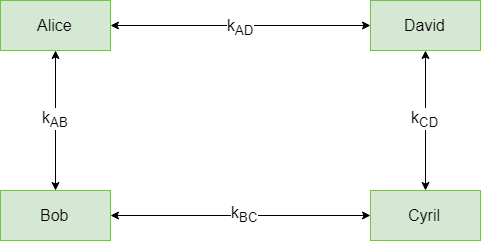
\includegraphics{img/AnonymesSenden.png}
\caption{AnonymesSenden.png}
\end{figure}

    \(k_{AB}=0001\)

\(k_{BC}=0010\)

\(k_{CD}=0011\)

\(k_{AD}=0100\)

\(M = 1101\)

Alice: \(k_{AB} + k_{AD} + M = 1000 = k_A\)

Bob: \(k_{AB} + k_{BC} = 0011 = k_B\)

Cyril: \(k_{BC} + k_{CD} = 0001 = k_C\)

David: \(k_{CD} + k_{AD} = 0111 = k_D\)

\(k_A + k_B + k_C + k_D = 1101 = M\)

    \subsection{Aufgabe 3: MIXe}\label{aufgabe-3-mixe}

    Spielen das anonyme Versenden von Nachrichten wie in Abschnitt 6.2
beschrieben anhand einfacher Zahlenbeispiele durch. Aufgabe: erstellen
Sie ein kurzes Protokoll (es soll ein von Ihnen durchgeführtes
Experiment beschreiben)!

    \begin{figure}
\centering
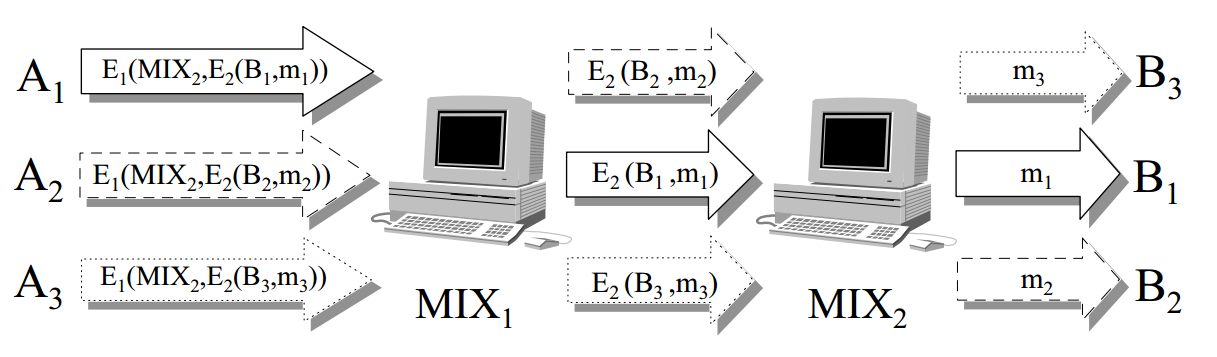
\includegraphics{img/mixe.png}
\caption{MIXe}
\end{figure}

    \begin{enumerate}
\def\labelenumi{\arabic{enumi}.}
\tightlist
\item
  A\_x verschlüsselt \(Message\) und \(Empfänger\) zu
  \(Cyphertext_1=E_2(B_1,m_1)\)
\item
  \(Cyphertext_1\) und Adresse von \(MIX_2\) wird verschlüsselt in
  \(Cyphertext_2=E_1(MIX_2,Cyphertext_1)\)
\item
  A\_x sendet \(Cyphertext_2\) an \(MIX_1\).
\item
  \(MIX_1\) kann den \(Cyphertext_2\) entschlüsseln zu \(Cyphertext_1\)
  und Empfänger \(MIX_2\). \(=> Cyphertext_2=D_1(MIX_2,Cyphertext_1)\)
\item
  \(MIX_1\) sendet \(Cyphertext_1\) zu \(MIXE_2\).
\item
  \(MIX_2\) kann den \(Cyphertext_1\) entschlüsseln zu \(Message\) und
  definitivem \(Empfänger=B_x\). \(=> Cyphertext_1=D_1(B,Message)\)
\item
  \(MIX_2\) sendet die \(Message\) zu B\_X.
\end{enumerate}

    \subsection{Aufgabe 4: Anonymität}\label{aufgabe-4-anonymituxe4t}

    Was ist «traffic analysis»? Welche Art von Anonymität, die Sie gelernt
haben, kann eine Lösung dagegen anbieten? Begründen Sie bitte Ihre
Antwort.

    "Traffic analysis is the process of intercepting and examining messages
in order to deduce information from patterns in communication, which can
be performed even when the messages are encrypted." - Wikipedia

Es ist also nichts anderes als eine MitM-Attacke auf eine Kommunikation.
Ein Zero-Knowledge Verfahren würde dabei helfen, da auf dem Kanal kein
Geheimnis übermittelt (und so nicht abgefangen werden kann). Trotzdem
können Sich die beiden Parteien gegeneinander authentifizieren.

Ebenfalls helfen würde der Einsatz von MIXen, da dort weder das
Identifizieren der Sender, Empfänger, oder Inhalt der Kommunikation
durch Abfangen von Nachrichten möglich ist.

    \subsection{Aufgabe 5: Secret Splitting / Geteiltes
Geheimnis}\label{aufgabe-5-secret-splitting-geteiltes-geheimnis}

    Verteilen Sie das Geheimnis 01011001 auf drei Leute! Protokollieren Sie
das Vorgehen und zeigen Sie, wie man das Geheimnis rekonstruiert.

    \(M = 01011001\)

Alice: \(11001100 = A\)

Bob: \(10101010 = B\)

Cyril: \(A + B + M = 00111111 = C\)

\(M = A + B + C = 01011001\)

    \subsection{Aufgabe 6: Secret Sharing Schema: Wie hoch ist das
Durchschnittsgehalt?
(OPTIONAL)}\label{aufgabe-6-secret-sharing-schema-wie-hoch-ist-das-durchschnittsgehalt-optional}

    Alice, Bob und Carol wollen jedoch nicht verraten, wie viel Geld sie
verdienen. Sie möchten jedoch den Durchschnitt ihrer Gehälter berechnen,
um mit Hilfe dieses Wertes zu ersehen, ob sie mit ihrem Gehalt zufrieden
sind oder ob sie bei der nächsten Gehaltserhöhung kräftig zulangen
sollten. Zunächst gehen sie mit einem kryptographischen Protokoll vor.
Alice startet. Sie wählt eine Zufallszahl \(r\) und addiert ihr Gehalt
\(a\) dazu. Diesen Wert schickt sie an Bob weiter. Er erhöht diesen Wert
um sein Gehalt \(b\). Dann fügt Carol Ihr Gehalt \(c\) dem vertraulichen
Wert \(r + a + b\) hinzu und gibt ihn an Alice zurück. 1. Wie berechnet
nun Alice den Durchschnitt ihrer Gehälter? 2. Kann eine/r der drei
Teilnehmenden das Gehalt einer/s anderen bestimmen? Begründen Sie bitte
Ihre Antwort? 3. Welche Werte kennt Bob?

    \begin{enumerate}
\def\labelenumi{\arabic{enumi}.}
\tightlist
\item
  Alice subtrahiert die Zufallszahl \(r\) und hat nun das Totalgehalt
  welches sie durch 3 teilt
\item
  Ein Teilnehmener kann nur das Durchschnitt- oder Totalgehalt der zwei
  anderen bestimmen
\item
  Bob kennt \(r+a\),sein Gehalt \(b\) und später der Durchschnitt
\end{enumerate}

    \subsection{Aufgabe 7: Threshold-Verfahren
(OPTIONAL)}\label{aufgabe-7-threshold-verfahren-optional}

    Alice teilt ein Geheimnis \(S\) mit einem Polynom des 2. Grades mit. Die
Zahl \(S\) ist die y-Achsenabschnitt (0, S), die das Geheimnis
darstellt. Als Teilgeheimnisse sind drei verschiedene Punkte
\((3, 2), (4, 1), (5, 2)\) bekannt. Wie rekonstruieren Sie das
Geheimnis?

    Allgemeines Polynom zweiten Grades:
\[f(x) = a_2\cdot x^2 + a_1\cdot x^1 + a_0\cdot 1\]

\[ 2 = a_2\cdot 3^2 + a_1\cdot 3^1 + a_0\cdot 1\]
\[ 1 = a_2\cdot 4^2 + a_1\cdot 4^1 + a_0\cdot 1\]
\[ 2 = a_2\cdot 5^2 + a_1\cdot 5^1 + a_0\cdot 1\]

\[
\begin{bmatrix}
2\\
1\\
2\\
\end{bmatrix}
=
\begin{bmatrix}
9 & 3 & 1\\
16 & 4 & 1\\
25 & 5 & 1\\
\end{bmatrix}
\cdot
\begin{bmatrix}
a_2\\
a_1\\
a_0\\
\end{bmatrix}
\]

\[
\begin{bmatrix}
a_2\\
a_1\\
a_0\\
\end{bmatrix}
=
\begin{bmatrix}
1\\
-8\\
17\\
\end{bmatrix}
\]

Und da \(S = a_0\) haben wir damit die Lösung \(S = 17\).

    \begin{Verbatim}[commandchars=\\\{\}]
{\color{incolor}In [{\color{incolor}9}]:} \PY{k+kn}{import} \PY{n+nn}{numpy} \PY{k}{as} \PY{n+nn}{np}
        \PY{n}{np}\PY{o}{.}\PY{n}{linalg}\PY{o}{.}\PY{n}{inv}\PY{p}{(}\PY{n}{np}\PY{o}{.}\PY{n}{matrix}\PY{p}{(}\PY{p}{[}\PY{p}{[}\PY{l+m+mi}{9}\PY{p}{,}\PY{l+m+mi}{3}\PY{p}{,}\PY{l+m+mi}{1}\PY{p}{]}\PY{p}{,}\PY{p}{[}\PY{l+m+mi}{16}\PY{p}{,}\PY{l+m+mi}{4}\PY{p}{,}\PY{l+m+mi}{1}\PY{p}{]}\PY{p}{,}\PY{p}{[}\PY{l+m+mi}{25}\PY{p}{,}\PY{l+m+mi}{5}\PY{p}{,}\PY{l+m+mi}{1}\PY{p}{]}\PY{p}{]}\PY{p}{)}\PY{p}{)}\PY{o}{*}\PY{n}{np}\PY{o}{.}\PY{n}{matrix}\PY{p}{(}\PY{p}{[}\PY{p}{[}\PY{l+m+mi}{2}\PY{p}{]}\PY{p}{,}\PY{p}{[}\PY{l+m+mi}{1}\PY{p}{]}\PY{p}{,}\PY{p}{[}\PY{l+m+mi}{2}\PY{p}{]}\PY{p}{]}\PY{p}{)}
\end{Verbatim}


\begin{Verbatim}[commandchars=\\\{\}]
{\color{outcolor}Out[{\color{outcolor}9}]:} matrix([[ 1.],
                [-8.],
                [17.]])
\end{Verbatim}
            
    \subsection{Aufgabe 8: Blinde Signatur}\label{aufgabe-8-blinde-signatur}

    Führen Sie zu Zweit die blinde Signatur durch. Protokollieren Sie das
Vorgehen und zeigen Sie, wie der Signierer die Nachricht berechnen kann,
welche er (blind) signiert!

    Bob:

\begin{itemize}
\tightlist
\item
  \(p = 3\)
\item
  \(q = 7\)
\item
  \(n = 3*7=21\)
\item
  \(e = 5\)
\item
  \(d = e^{-1}=17\)
\end{itemize}

Alice:

\begin{itemize}
\tightlist
\item
  \(k=13\)
\item
  \(M=10\)
\item
  \(t = M*k^e = 10*13^5 = 4 \mod 21\)
\end{itemize}

Bob:

\begin{itemize}
\tightlist
\item
  \(u = t^d = 4^{17} = 16 \mod 21\)
\end{itemize}

Alice:

\begin{itemize}
\tightlist
\item
  \(M^d = u*k^{-1} = 16 * 13^{-1} = 19 \mod 21\)
\end{itemize}


    % Add a bibliography block to the postdoc
    
    
    
    \end{document}
